\newcommand{\notenumber}{2019-xx}
\newcommand{\notetitle}{Background for \acp{pcm} for intense electron beam driven plasmas*}
\newcommand{\noteauthors}{P.~E.~Adamson}
\newcommand{\noteabstract}{Various \acp{pcm} are developed for intense electron
beam driven plasmas in Ar and air (dry and wet).  This work is part of an effort to 
develop \acp{prm} for a DTRA- and NRL-funded effort to update ICEPIC and MEEC++ to
model \ac{sgemp}.}
%TODO: if new calcs, describe...
%TODO: if new data from literature, describe...
%TODO: If different decisions, describe...
%TODO: How will model be V&V'd?
\newcommand{\notesponsor}{DTRA/RD-NTE 6.2 program}

%TODO: use mhchem for all chemical species/equations
\documentclass[12pt]{article}
\usepackage{graphicx}
\usepackage{amsmath}
\usepackage{amssymb}
\usepackage{amscd}
\usepackage{siunitx}
\usepackage{bbm}
\usepackage{epstopdf}
\DeclareGraphicsRule{.tif}{png}{.png}{`convert #1 `dirname #1`/`basename #1 .tif`.png}
\usepackage{color,soul}
\usepackage{rotating}
\usepackage{multirow}
\usepackage[htt]{hyphenat}
\usepackage[version=4]{mhchem}
\usepackage{subfigure}
\usepackage{dcolumn}
\usepackage{wrapfig}
\usepackage[nolist,nohyperlinks]{acronym}
\usepackage{array}
%\usepackage{parskip}
%\parskip=1em
\usepackage{verbatimbox}

\newcommand*{\restrictlinewidthbox}[1]{%
  \begingroup
    \sbox0{#1}%
    \ifdim\wd0>\linewidth
      \resizebox{\linewidth}{!}{\copy0}%
    \else
      \copy0 %
    \fi
  \endgroup
}

\newcolumntype{d}[1]{D{.}{.}{#1}}
\newcommand\mc[1]{\multicolumn{1}{c}{#1}}
\newcommand{\vect}[1]{\boldsymbol{#1}}

%\usepackage{tikz,pgfplots}
%\pgfplotsset{compat=newest} 
%\pgfplotsset{plot coordinates/math parser=false}

% for better list... used for custom title page
\usepackage{enumitem}

%\usepackage{pgf}
%\usepackage{pgffor}
%\usepgflibrary{plothandlers}

%\usepgfplotslibrary{external} 
%\tikzexternalize% activate externalization!

% use this to remake a particular plot...
%\tikzset{external/remake next}

%use this to remake all
%\tikzset{external/force remake}

%\tikzsetexternalprefix{figures/}

%% Fonts %%
\usepackage{microtype}

\usepackage[T1]{fontenc}
\usepackage{textcomp}

% Times New Roman
\usepackage{mathptmx}

% this stuff is to make the section headings look like phys plasmas
\usepackage[scaled=.92]{helvet}
%\usepackage{helvet}

% NB, use citenum to get inline citation (not superscript)

\usepackage[colorlinks=true,
		citecolor=blue,
		linkcolor=blue,
		anchorcolor=blue,
		filecolor=blue,
		menucolor=blue,
		runcolor=blue,
		urlcolor=blue,
		unicode
		]{hyperref}
\usepackage[all]{hypcap}

%
\usepackage{geometry}
\geometry{margin=1in}

\usepackage{sectsty}  
%\sectionfont{\normalfont\sffamily\large\underline\bfseries\color{orange}}
%\sectionfont{\normalfont\sffamily\large\bfseries\color{orange}\sectionrule{0pt}{??0pt}{-4pt}{1pt}}
%\sectionfont{\normalfont\sffamily\large\bfseries\sectionrule{3ex}{3pt}{-1ex}{1pt}}
\sectionfont{\normalfont\sffamily\large\bfseries}
\subsectionfont{\normalfont\sffamily\normalsize\bfseries}

\newcommand{\mycomment}[1]{}
\newcommand{\tbd}{\textcolor{red}{\textbf{\hl{TBD}}}}

% set noindents for entire document
\setlength\parindent{0pt}
%\setlength{\parskip}{1em}

\newcolumntype{P}[1]{>{\centering\arraybackslash}p{#1}}

%%%%%%%%%%%%%%%%%%%%%%%%%%%%%%%%%%%%%%%%%%%%
%% BEGIN DOCUMENT
%%%%%%%%%%%%%%%%%%%%%%%%%%%%%%%%%%%%%%%%%%%%
\begin{document}
/Users/adamson/projects/latex/acronyms.tex
\graphicspath{{./fig/}}
\begin{titlepage}

\rmfamily
\begin{center}\sffamily\bfseries
PULSED POWER PHYSICS TECHNOTE NO. \notenumber{}\\
{~}
\end{center}

\begin{description}[leftmargin=8em,style=nextline,font=\sffamily\bfseries ]
\item[TITLE:]{\bfseries 
\notetitle{}
}
\item[AUTHORS:]{ \noteauthors{}\\
{\itshape Code 6770, Plasma Physics Division, Naval Research Laboratory}}
\item[DATE:]\today
\item[ABSTRACT:] 
\noteabstract{}
\end{description}

\vfill

{\small
\noindent THIS REPORT REPRESENTS UNPUBLISHED INTERNAL WORKING DOCUMENTS AND SHOULD NOT BE REFERENCED OR DISTRIBUTED WITHOUT THE AUTHORS' CONSENT

{~}

\noindent * Work supported by \notesponsor{}. 
}
\end{titlepage}

\pagestyle{myheadings}



\markright{\hfill \color{red}\sf DRAFT VERSION DO NOT CIRCULATE \hfill}

\section{Introduction}

\begin{figure}
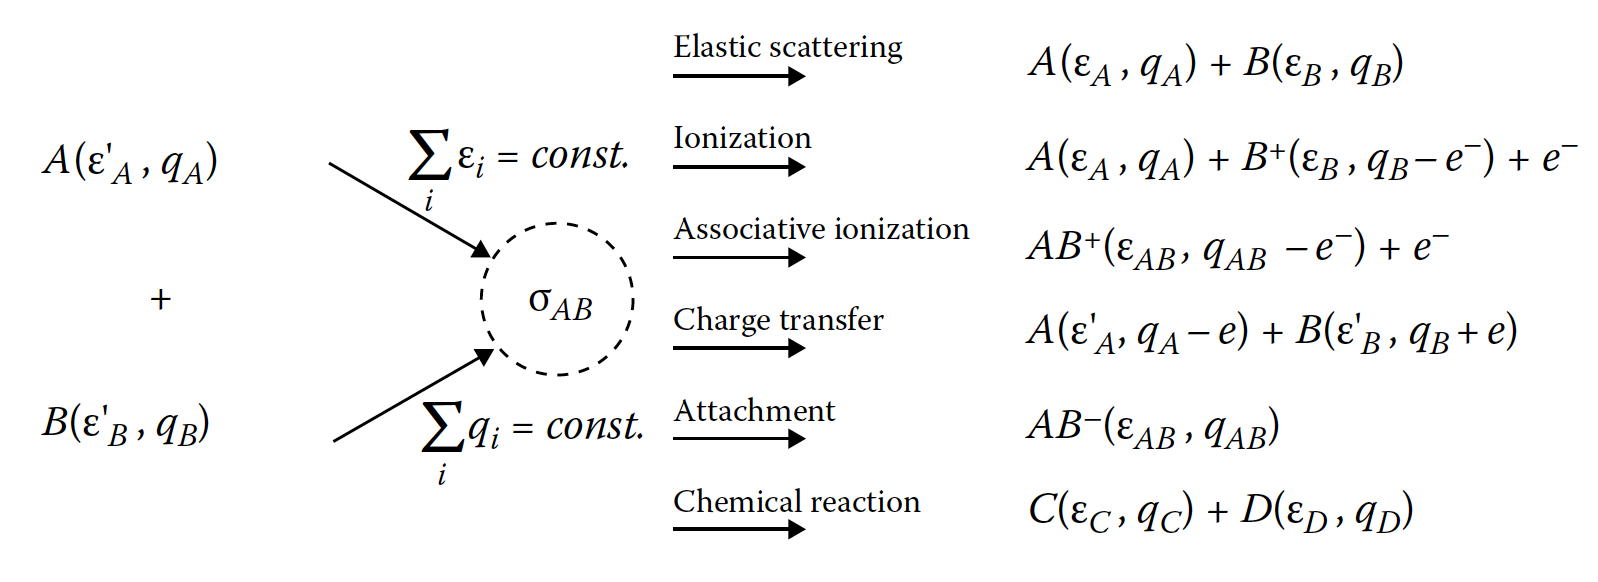
\includegraphics[width=.9\textwidth]{meichsner_fig3.7.eps}
\caption{Important elementary collision processes between particles in the plasma volume 
with collision cross section $\sigma_{AB} (\epsilon)$ ($A, B$: particles with total energy 
$\epsilon$ and charge $q$; $e$: elementary charge).\cite{meichsner2013}}
\end{figure}

\begin{figure}
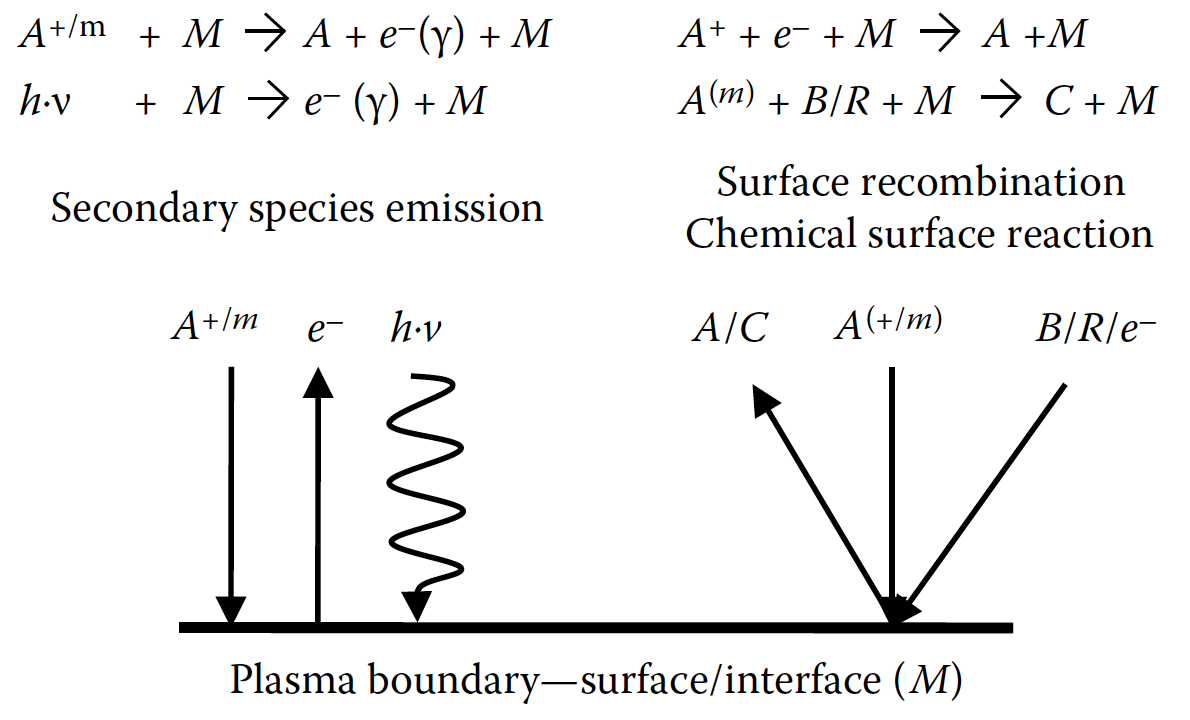
\includegraphics[width=0.6\textwidth]{meichsner_fig3.8.eps}
\caption{Important elementary collision processes on the surface, $A^{+/m}$ : ion/metastable;
$R$: radical; $h \cdot \nu$: photon; $e^−$ : electron; $A, B, C$: atom or molecule; $M$: surface.\cite{meichsner2013}}
\end{figure}

\begin{table}
\caption{Overview and the Classification of the Different Elementary Collision
Processes of Electrons in the Plasma Volume}
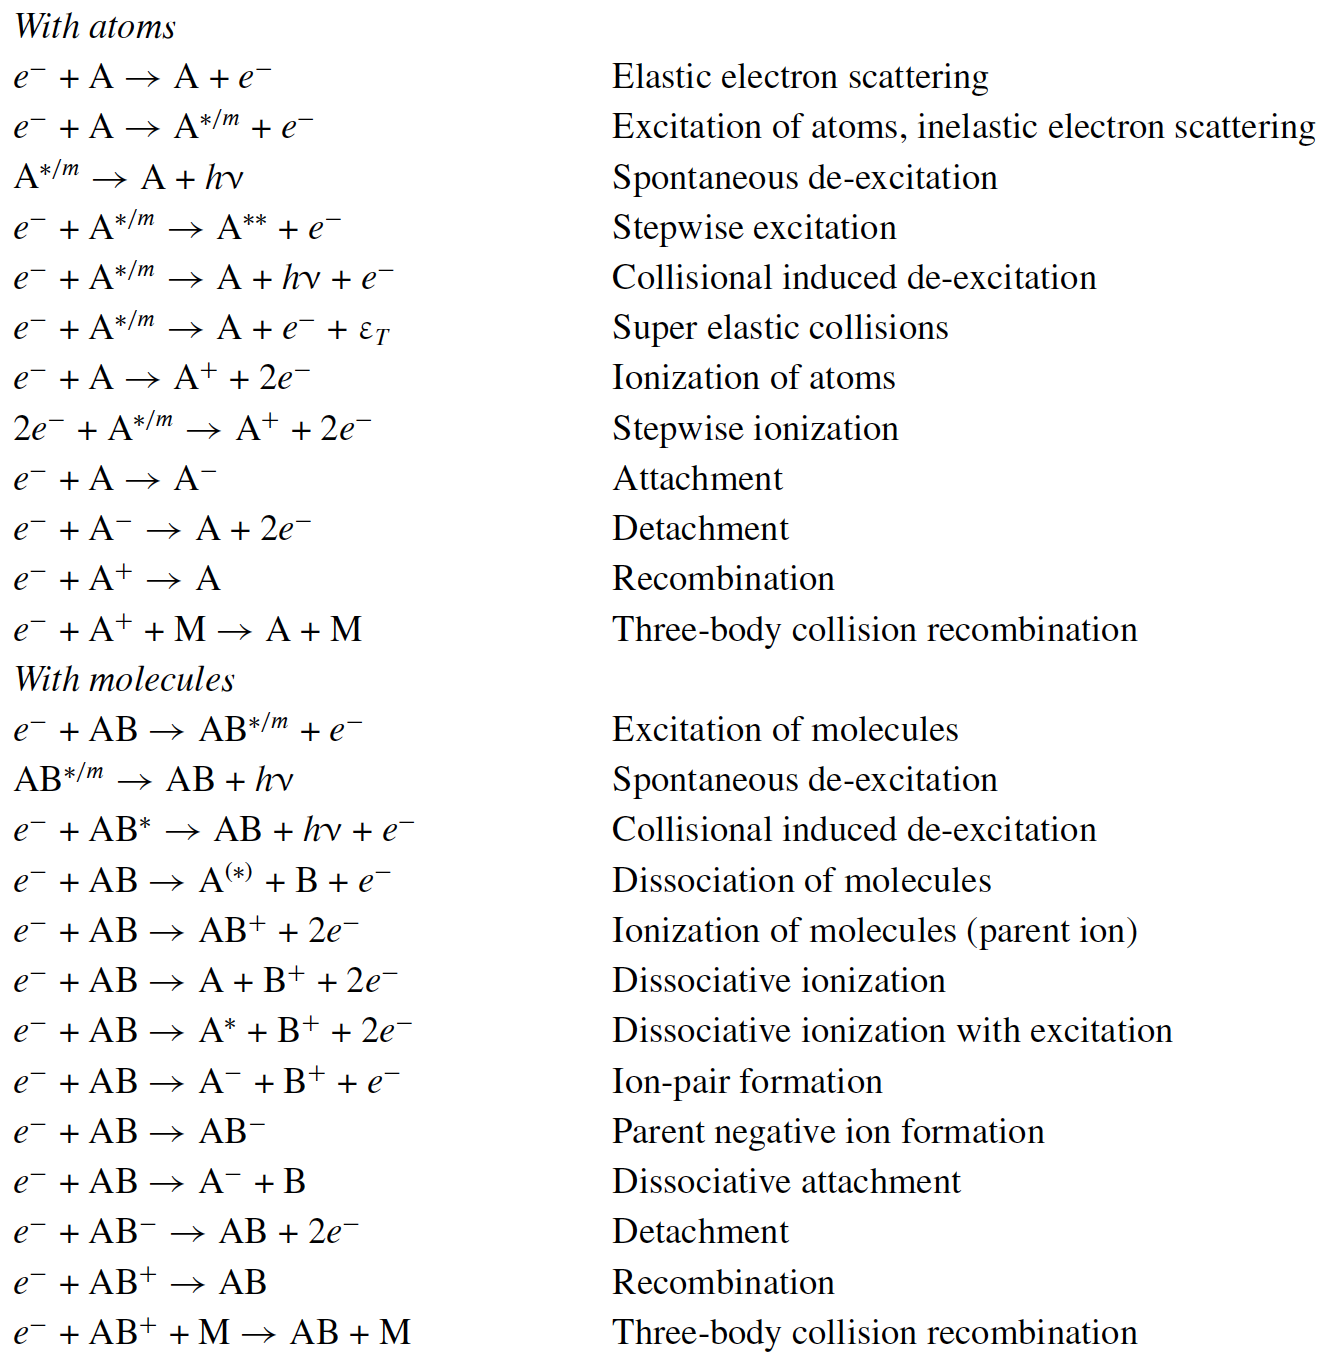
\includegraphics[width=0.6\textwidth]{meichsner_tab3.7.eps}
\end{table}

\begin{table}
\caption{Overview and the Classification of the Different Elementary Collision
Processes of Heavy Particles in the Plasma Volume}
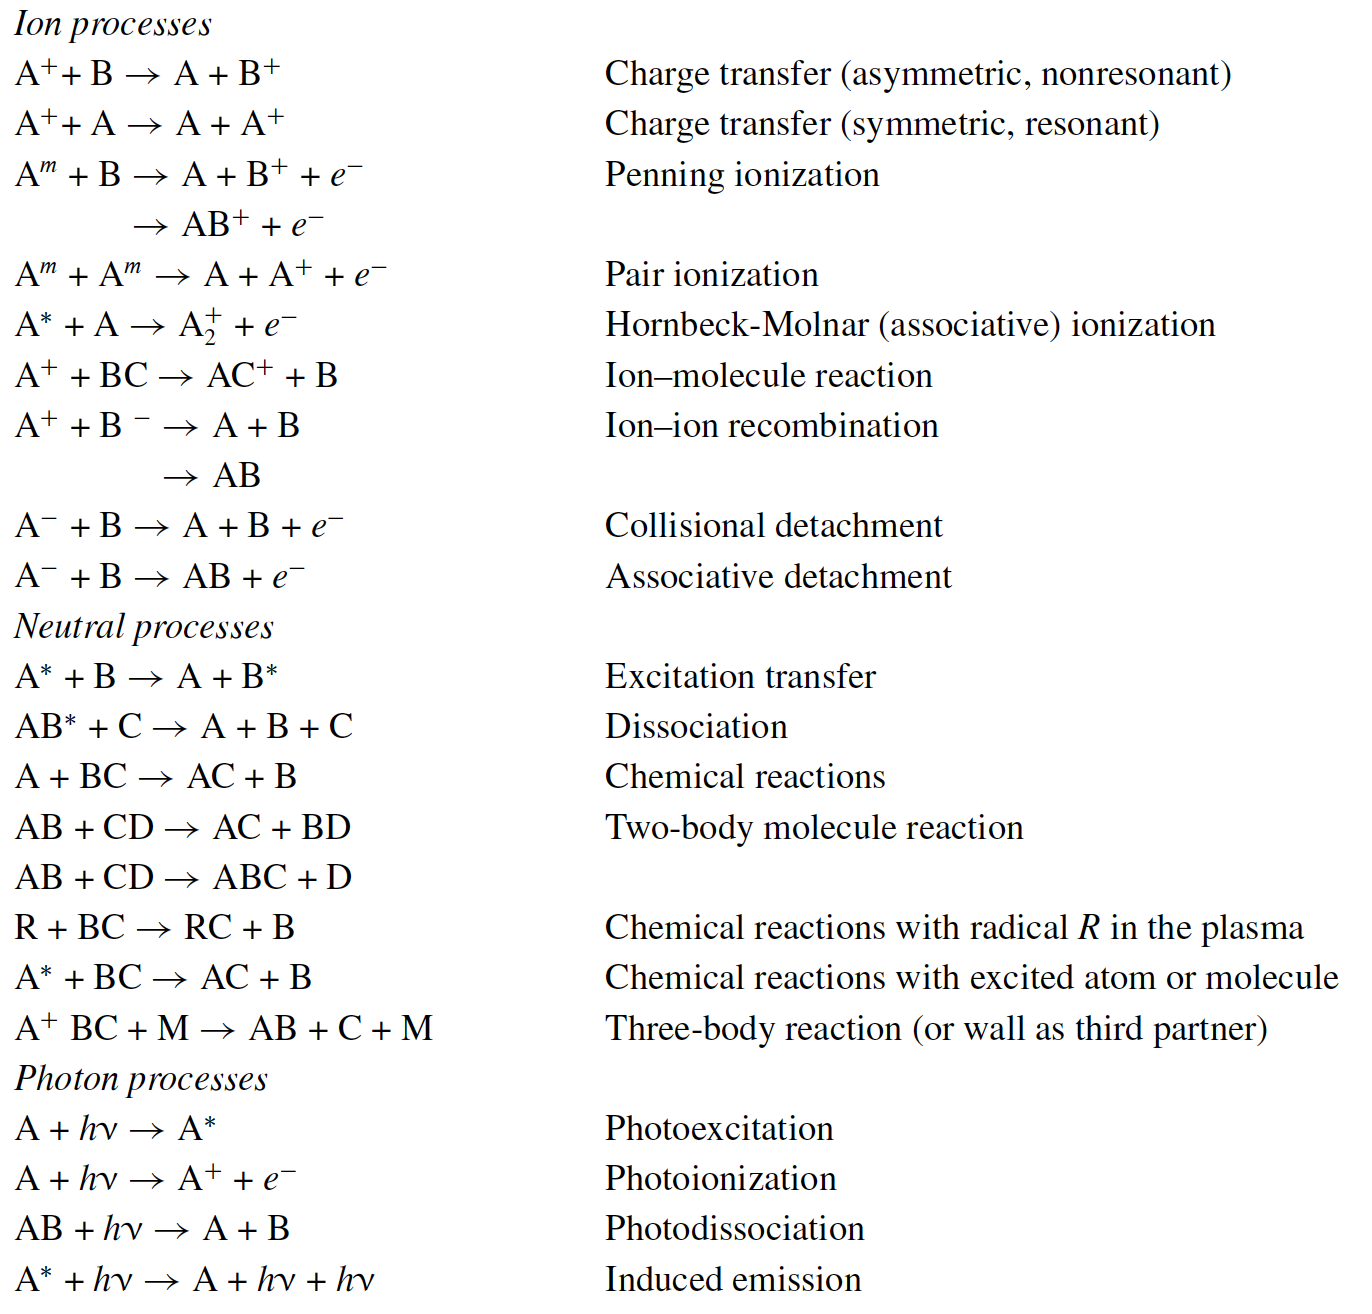
\includegraphics[width=0.6\textwidth]{meichsner_tab3.8.eps}
\end{table}

For the designation of the electronic energy levels of atoms and diatomic
molecules the spectroscopic notation is used:\\

\begin{itemize}
\item Atom: $nl^w\; {}^{2S+l}L_j$\\
\item Diatomic molecule: $nl^w\; {}^{2S+l}\Lambda_\Omega$
\end{itemize}
 
with the main quantum number $n$, the angular momentum $l$, the number of electrons
in the shell $w$, the resulting spin $S$, the multiplicity $2S + 1$, the resulting angular
momentum $L$ ($L = 0, 1, 2,...$ corresponding to energy levels indicating the $S, P, D,. . .$ 
states), the total angular momentum $J = L+S$ which represents the  $LS$ coupling in
the case of light atoms, and in the case of diatomic molecules  $\Omega =\Lambda + \sum_{g,u}^{+,-}$ represents
the projection of the corresponding momentum vectors onto the internuclear axis in
Greek letters with the addition + or – as well as $g$ or $u$ describing the symmetry
properties of the electronic wave function. The convention for the state assignment in
molecules are $X$ for the ground state, $A, B,\ldots$ for excited states of the same multiplicity
as the ground state $X$, and $a, b,\ldots$ for excited states of different multiplicity as $X$.

Tables and figures to include in each PCM:

\begin{itemize}
\item permitted radiative transitions in neutral atoms
\item potential energy curves
\item metastable energy levels
\item electron impact ionization thresholds
\item dissociative electron attachment thresholds
\end{itemize}


\bibliography{ref}{}
\bibliographystyle{unsrt}

\end{document}

\endinput



